% soctepmlate unofficial - SOČ = Středoškolská odborná činnost - Czech competition
% Author: Vojtěch Boček
% Edit by: Jaroslav Páral
% Version: 2018-02-12
% Source code: https://github.com/RoboticsBrno/soctemplate/
% Base on: http://www.jcmm.cz/cz/sablona-soc.html
% License: CC BY 4.0
% Edited by: Pavel Šrytr for his SOC team needs and to meets the requierements of the SOC supervisor
% Further edited by Jakub Hampl


\documentclass{socthesis}

\usepackage{subcaption}
\usepackage{amsmath}
\usepackage{enumitem}
\usepackage[T1]{fontenc}
\usepackage{hyperref}
\usepackage{siunitx}
\usepackage{float}
\usepackage{titlesec}
\usepackage[bottom, hang, flushmargin]{footmisc}
\usepackage{xcolor}
\usepackage{listings}
\definecolor{mGreen}{rgb}{0,0.6,0}
\definecolor{mGray}{rgb}{0.5,0.5,0.5}
\definecolor{mPurple}{rgb}{0.58,0,0.82}
\definecolor{backgroundColour}{rgb}{0.95,0.95,0.92}
\definecolor{dkpurple}{rgb}{0.5, 0, 0.5}
\definecolor{dkblue}{rgb}{0,0,.6}
\definecolor{dkyellow}{cmyk}{0,0,.8,.3}

\lstdefinestyle{CStyle}{
    backgroundcolor=\color{backgroundColour},   
    commentstyle=\color{mGreen},
    keywordstyle=\color{magenta},
    numberstyle=\tiny\color{mGray},
    stringstyle=\color{mPurple},
    basicstyle=\footnotesize,
    breakatwhitespace=false,         
    breaklines=true,                 
    captionpos=b,                    
    keepspaces=true,                 
    numbers=left,                    
    numbersep=5pt,                  
    showspaces=false,                
    showstringspaces=false,
    showtabs=false,                  
    tabsize=2,
    language=C
}

\lstdefinestyle{PHPStyle}{
    language= php,
    basicstyle= \small\ttfamily,
    keywordstyle= \color{dkblue},
    stringstyle= \color{mGreen},
    identifierstyle=\color{dkpurple},
    commentstyle= \color{gray},
    emph=[1]{php},
    emphstyle=[1]\color{black},
    emph=[2]{if,and,or,else,public,function,new,return},
    emphstyle=[2]\color{dkyellow}
}

\lstdefinestyle{PythonStyle}{
    backgroundcolor=\color{backgroundColour},   
    commentstyle=\color{mGreen},
    keywordstyle=\color{magenta},
    numberstyle=\tiny\color{mGray},
    stringstyle=\color{mPurple},
    basicstyle=\footnotesize,
    breakatwhitespace=false,         
    breaklines=true,                 
    captionpos=b,                    
    keepspaces=true,                 
    numbersep=5pt,                  
    showspaces=false,                
    showstringspaces=false,
    showtabs=false,                  
    tabsize=2,
    language=Python
}
\renewcommand{\lstlistingname}{Program}
\renewcommand{\lstlistlistingname}{Seznam programů}
\usepackage[left=3.5cm, right=2.5cm, top=2.5cm, bottom=2.5cm]{geometry}

\newcommand*{\noaddvspace}{\renewcommand*{\addvspace}[1]{}}
\addtocontents{lof}{\protect\noaddvspace}

\interfootnotelinepenalty=10000
\pretolerance=150
\setlength{\emergencystretch}{3em}

\usepackage{chngcntr}
\counterwithout{footnote}{chapter}

\addbibresource{text.bib}

\titlecz{Rozřazovák -- jazykový rozřazovací test}
\titleen{Rozřazovák -- language placement test}
\author{Jakub Hampl}
\field{12}
\school{Gymnázium Jana~Palacha, Pod Vrchem 3421, Mělník 276 01}
\mentor{Mgr. Markéta Wolfová}
\mentorstatement{Mgr. Markétě Wolfové}


\begin{document}
\titleformat
{\chapter} % command
[hang] % shape
{\normalfont\huge\bfseries} % format
{\thechapter} % label
{0ex} % sep
{
    \vspace{-2ex}
} % before-code
[
    \vspace{1ex}
] % after-code
	\maketitle
	\makecopyrightstatement{Mělník}
	
	\makethanks{Především děkuji Marianu Šámalovi -- za jeho mentorství a ochotu, za jeho specifický smysl pro humor a za to, že ten test tenkrát odevzdal třikrát.
	
	Dále děkuji Mgr. Markétě Wolfové a PaedDr. Daně Hilské za jejich práci při robotickém kroužku, kde se díky nim rozvíjí mnoho nadějných talentů.}
	
	\pagestyle{empty}
	
	\section*{Anotace}
    Ve své práci se věnuji tvorbě moderní webové aplikace za účelem testování žáků pro jejich rozdělení do jazykových skupin.
	
	\subsection*{Klíčová slova}
	edukační software, webová aplikace, rozřazovací test
	
	\vspace{20mm}
	
	\section*{Annotation}
    In my work I talk about the creation of a modern web application for the purpose of testing students for placing them into language groups.
	
	\subsection*{Keywords}
	education software, web application, placement test
	
	\titlespacing{\chapter}{0pt}{0cm}{0pt}
	\titlespacing{\section}{0pt}{0cm}{0pt}
	\titlespacing{\subsection}{0pt}{0pt}{0pt}
	
	\newpage
	\pagestyle{plain}
	\pagenumbering{gobble}
    \tableofcontents % vysází obsah
	
	%%% Začátek práce
	\setcounter{figure}{0}
	\setcounter{table}{0}
	\newpage
	
	%%% Úvod
	\pagenumbering{arabic}
	\setcounter{page}{9}
	\chapter*{Úvod}
\addcontentsline{toc}{chapter}{Úvod} % přidá položku úvod do obsahu

Jako kdyby to bylo včera, když jsem pár let zpátky u nás na gymnáziu podstoupil takzvaný \enquote{rozřazovák} -- test, který nás měl podle našich znalostí angličtiny rozdělit do několika jazykových skupin. Program, ve kterém jsme pracovali, byl zastaralý už jen od pohledu a šel triviálně rozbít. Taky si dobře vzpomínám, jak do dveří vtrhla učitelka angličtiny a začala hubovat spolužáka, \textit{proč ten test odevzdal třikrát?}

Program nakonec přestal fungovat úplně. Od té doby se poslechová část dělá na papír a zbytek na počítači, což je nepohodlné nejen pro žáky, ale hlavně pro učitele. Rozhodl jsem se ho tedy přetvořit. Mým cílem je vytvořit program, který bude generovat originální testy každému žákovi, dokáže spolehlivě otestovat desítky lidí naráz a výsledky automaticky zpracovat. Měl by používat nejmodernější volně dostupné technologie, být intuitivní a hlavně život žákům i učitelům usnadnit, ne naopak.
	
	
	%%% Obsah
	\hypertarget{Design}{\chapter{Design}}

\section{Motivace}

Při tvorbě aplikace bylo neustále nutné myslet na dva hlavní faktory, kolem kterých se celý design musí odvíjet; to sice, že je program mířený pro dvě skupiny: učitele a žáky zároveň. 

Úkolem žáka je v časovém limitu odpovědět na jazykové otázky. Žák by měl mít co nejméně možností, jak podvádět, aby byl správně umístěn do jazykové skupiny úměrné jeho znalostem; dostane náhodnou sadu otázek různých obtížností, které pro jeho ročník navolí učitel.

Učitel pracuje se svým vlastním rozhraním, kde zadává otázky, vytváří testy, kontroluje průběh testování a získává automaticky zpracované výsledky.

V obou případech je důležité, aby byla webová aplikace intuitivní na používání, měla příjemný design a hlavně spolehlivě fungovala.

\section{Přihlašování}
\label{sec:login-design}

Ještě před tím, než se uživatelé dostanou do svého rozhraní, je potřeba, aby se přihlásili. Tato část aplikace je společná pro žáky i učitele. 

\begin{figure}[H]
    \centering
    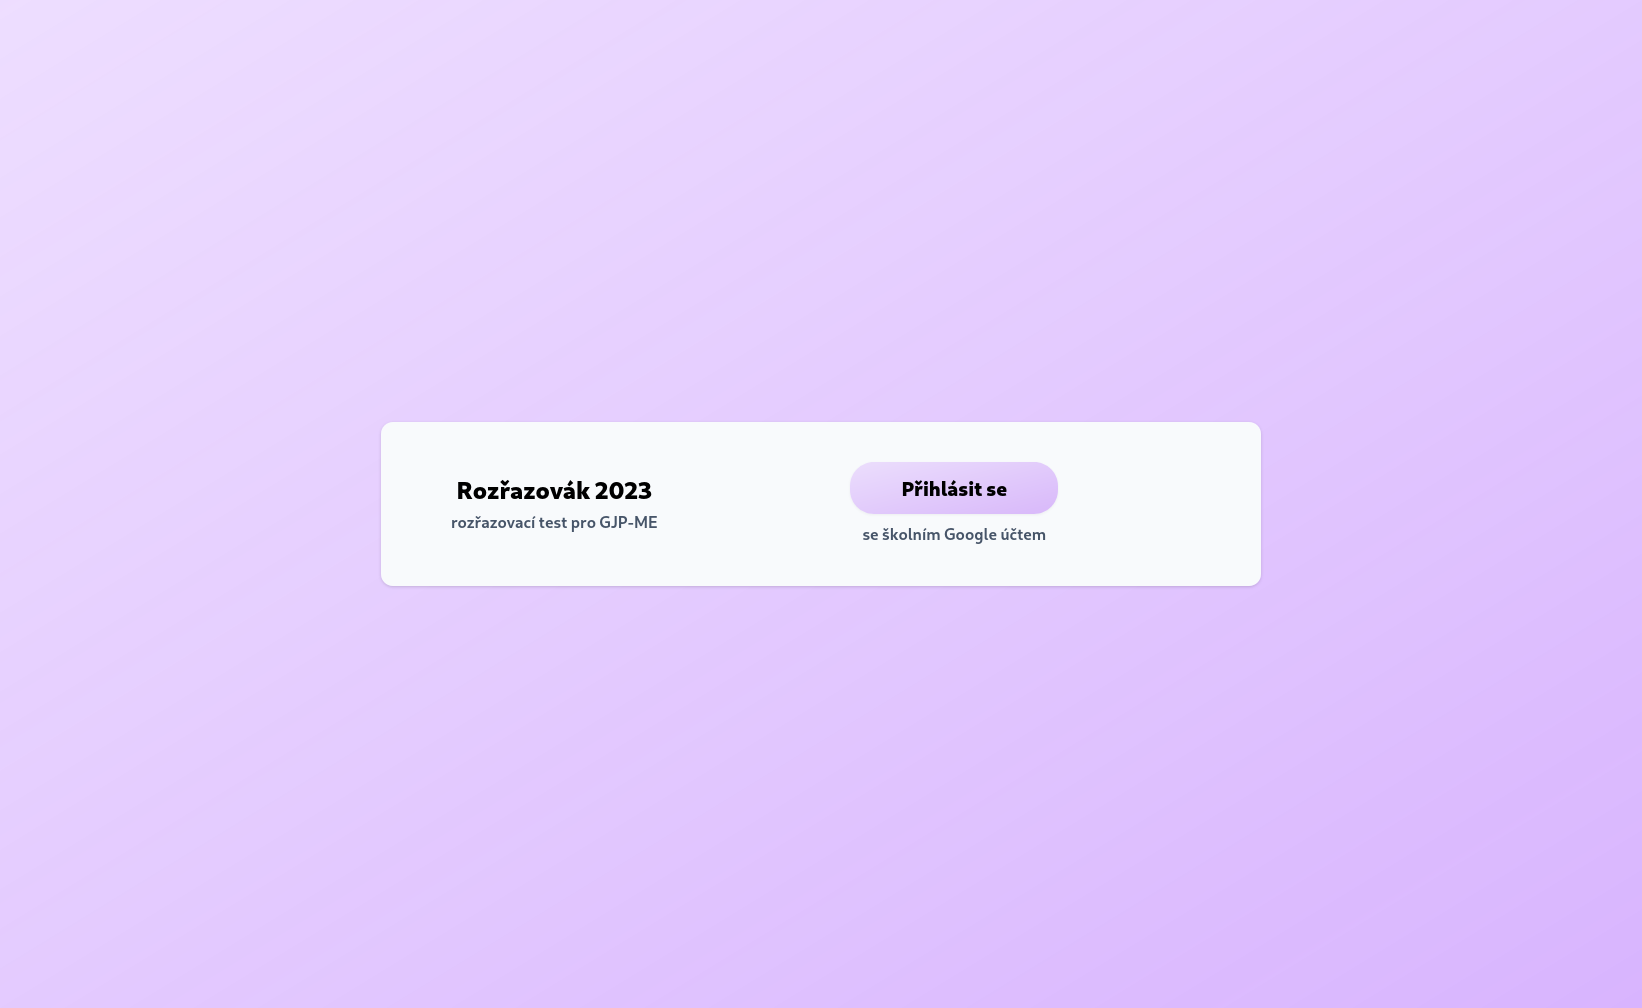
\includegraphics[width=350px]{images/01design/login.png}
    \caption{Přihlašovací stránka je hlavní stránkou aplikace.}
\end{figure}

Učitelé a žáci se přihlásí pomocí svého školního Google účtu (vizte \ref{sec:login}).

\newpage

Pokud se přihlásí učitel, zobrazí se nabídka pro přechod do administrátorské sekce.

\begin{figure}[H]
    \centering
    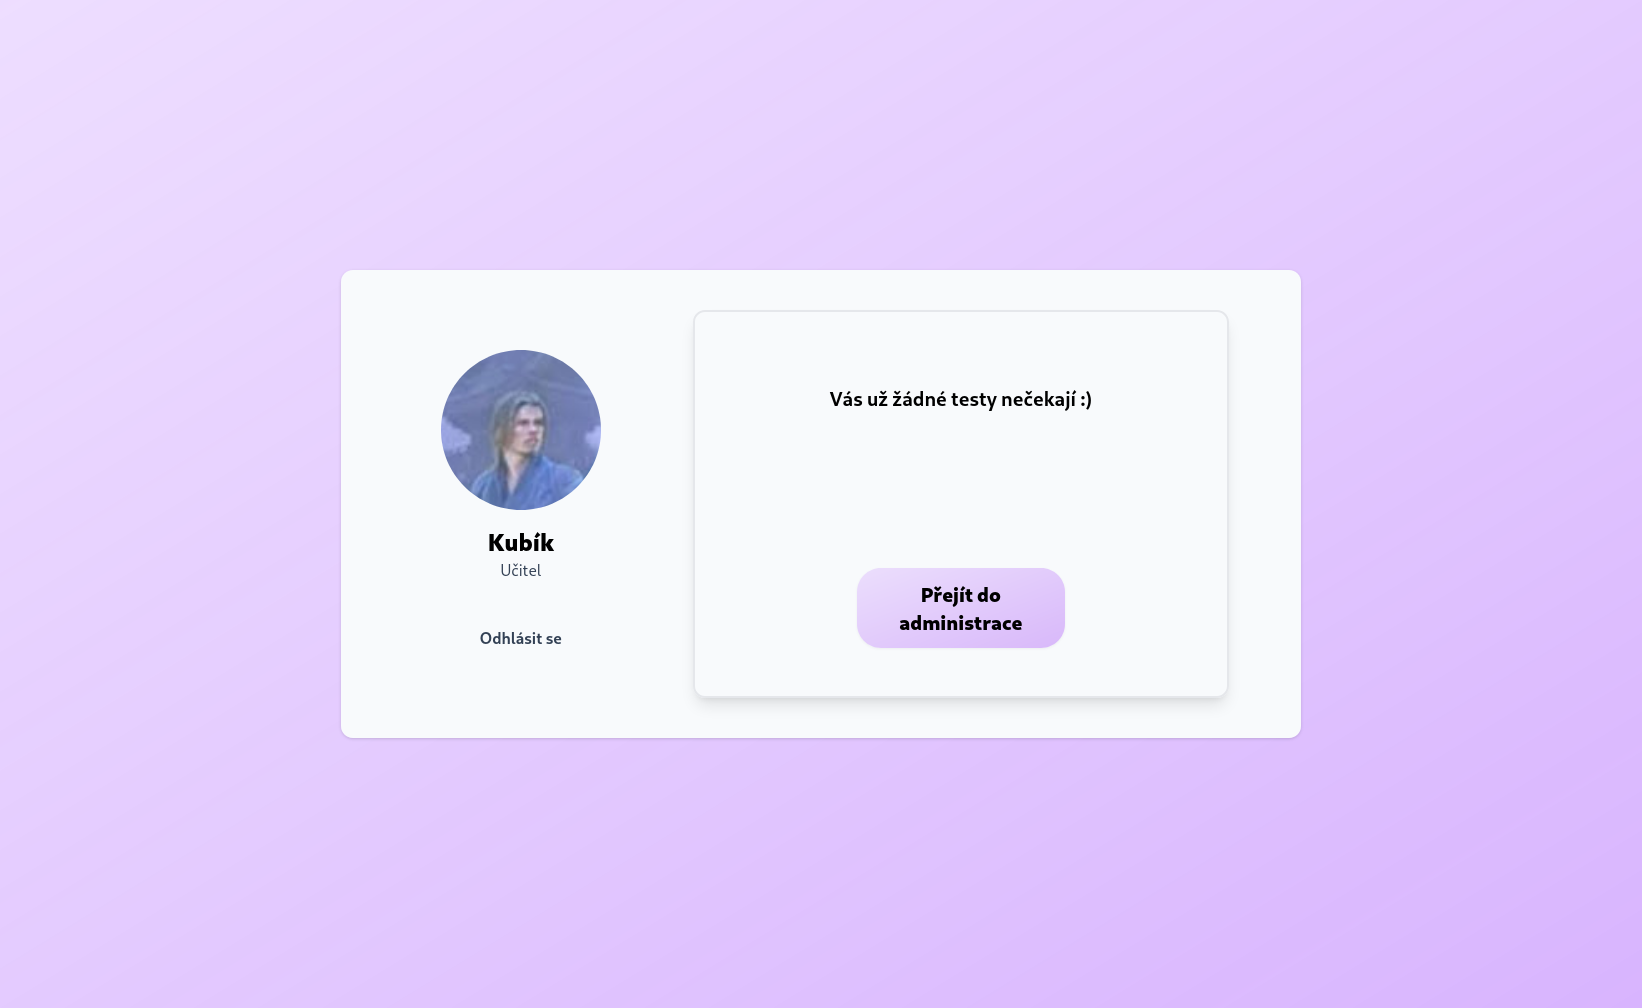
\includegraphics[width=350px]{images/01design/teacher.png}
    \caption{Hlavní stránka po přihlášení učitele.}
\end{figure}

Pokud se přihlásí žák, ve výchozím stavu se mu zobrazí stránka s informací, že pro něj aktuálně není spuštěný žádný test.

\begin{figure}[H]
    \centering
    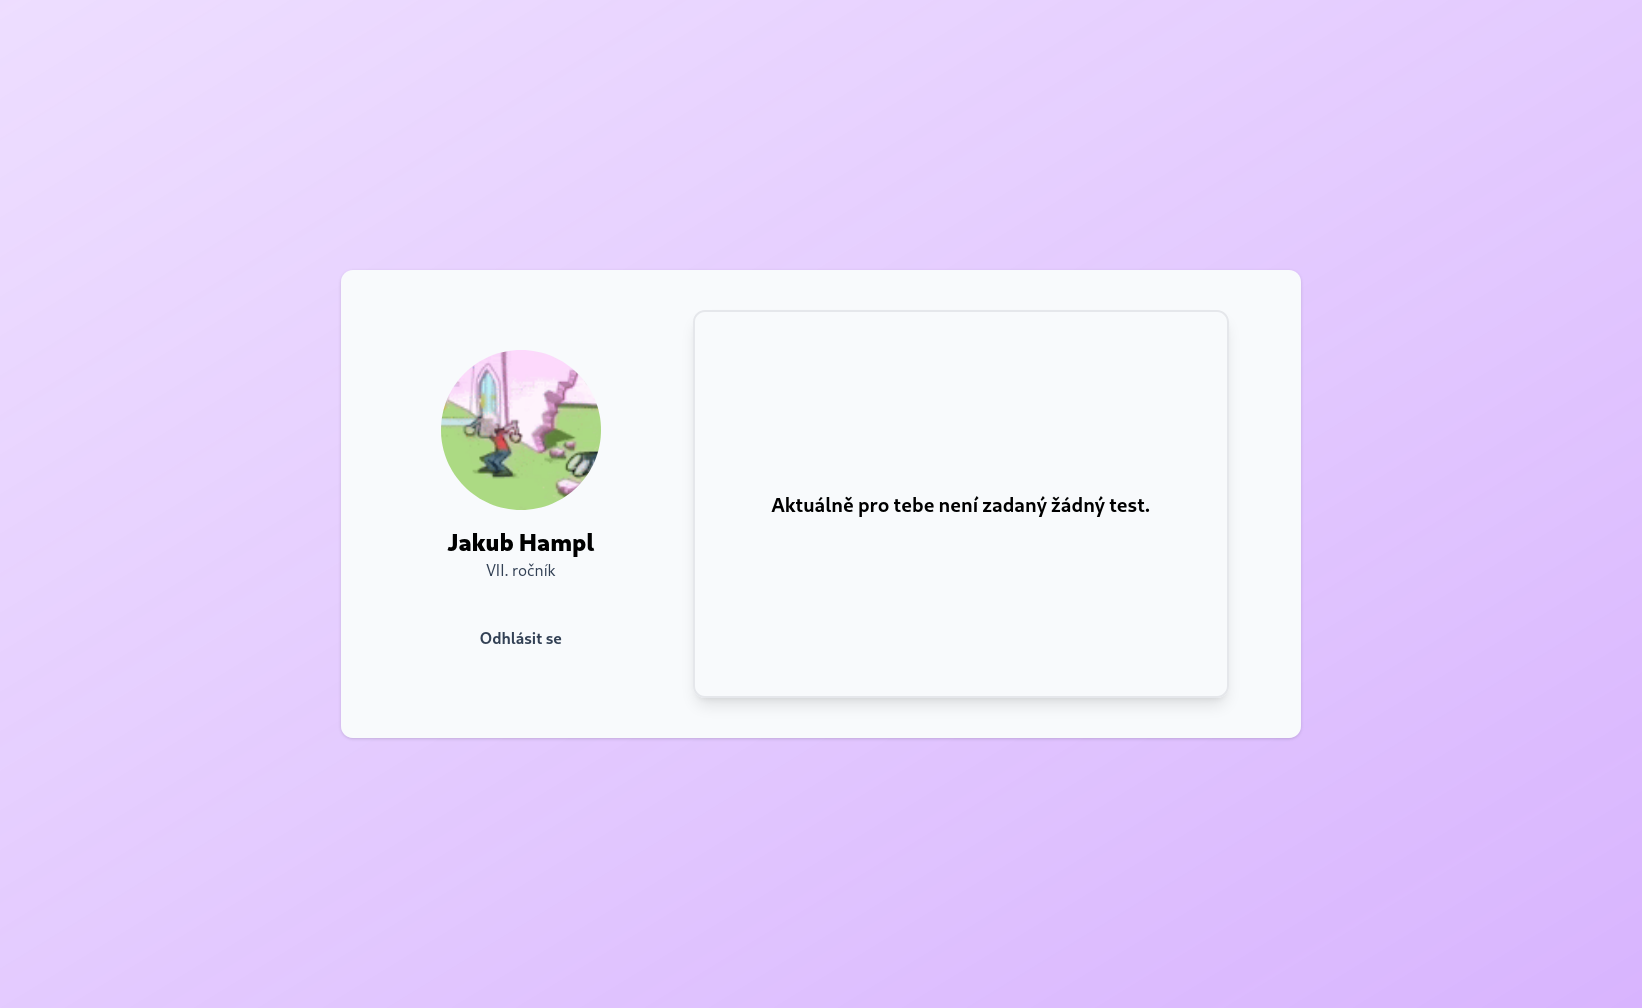
\includegraphics[width=350px]{images/01design/student-no-test.png}
    \caption{Hlavní stránka po přihlášení žáka bez zadaného testu.}
\end{figure}

Pokud je pro ročník přihlášeného žáka aktuálně aktivovaný test, je vidět jeho časové omezení, počet otázek a obtížnost. Pokud ne, zobrazí se pouze informace o tom, že pro žáka žádný test aktuálně spuštěný není.

\begin{figure}[H]
    \centering
    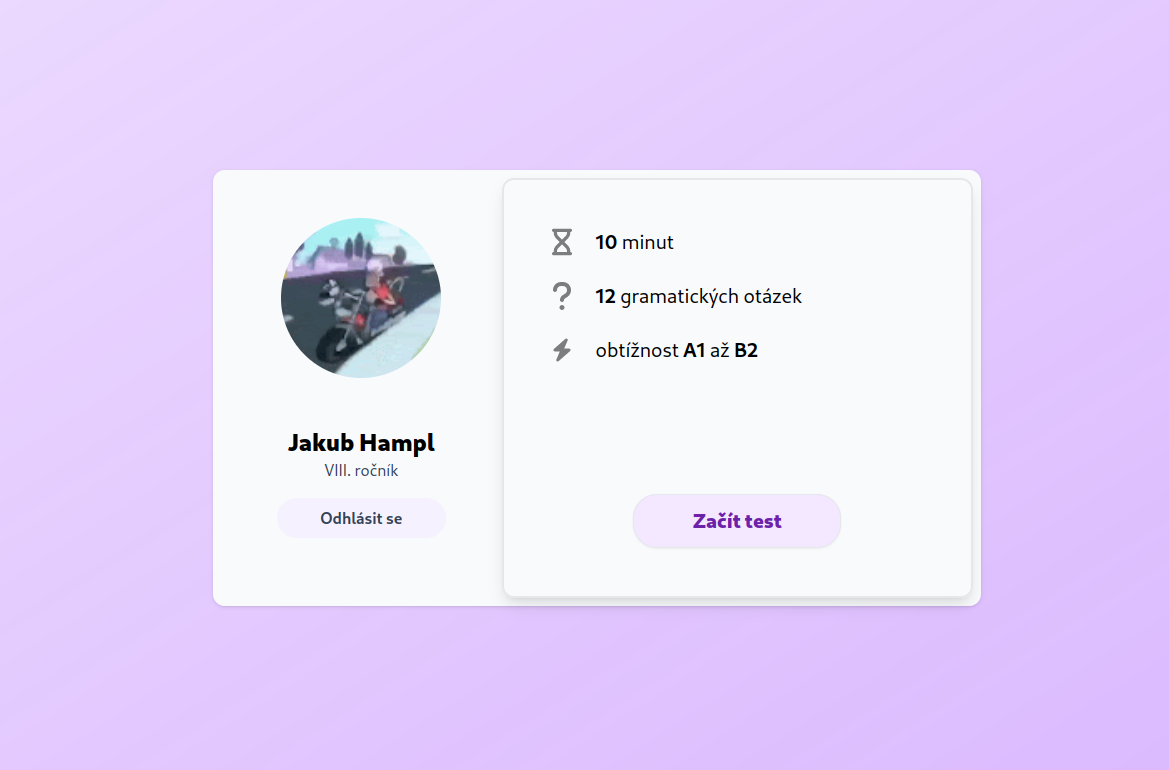
\includegraphics[width=350px]{images/01design/student-yes-test.png}
    \caption{Hlavní stránka po přihlášení žáka se zadaným testu.}
\end{figure}

Při aktivovaném testu může žák test spustit. Po spuštění se pro žáka vygeneruje originální sada otázek (vizte ODKAZ) a žák je přesměrován do žákovského rozhraní. Pokud žák během testu tuto stránku opustí (například kvůli technickým potížím, výpadku proudu, atp.), zůstává test spuštěný a je možné pokračovat v jeho vyplňování z hlavní stránky. 

\begin{figure}[H]
    \centering
    
\includegraphics[width=200px]{images/01design/continue.png}
    \caption{Při probíhajícím testu se text tlačítka změní na "Pokračovat" a zobrazí se pod ním zbývající čas.}
\end{figure}

Jakmile žák test odevzdá, je přesměrován zpět na hlavní stránku, kde mu je sdělen jeho výsledek.

\begin{figure}[H]
    \centering
    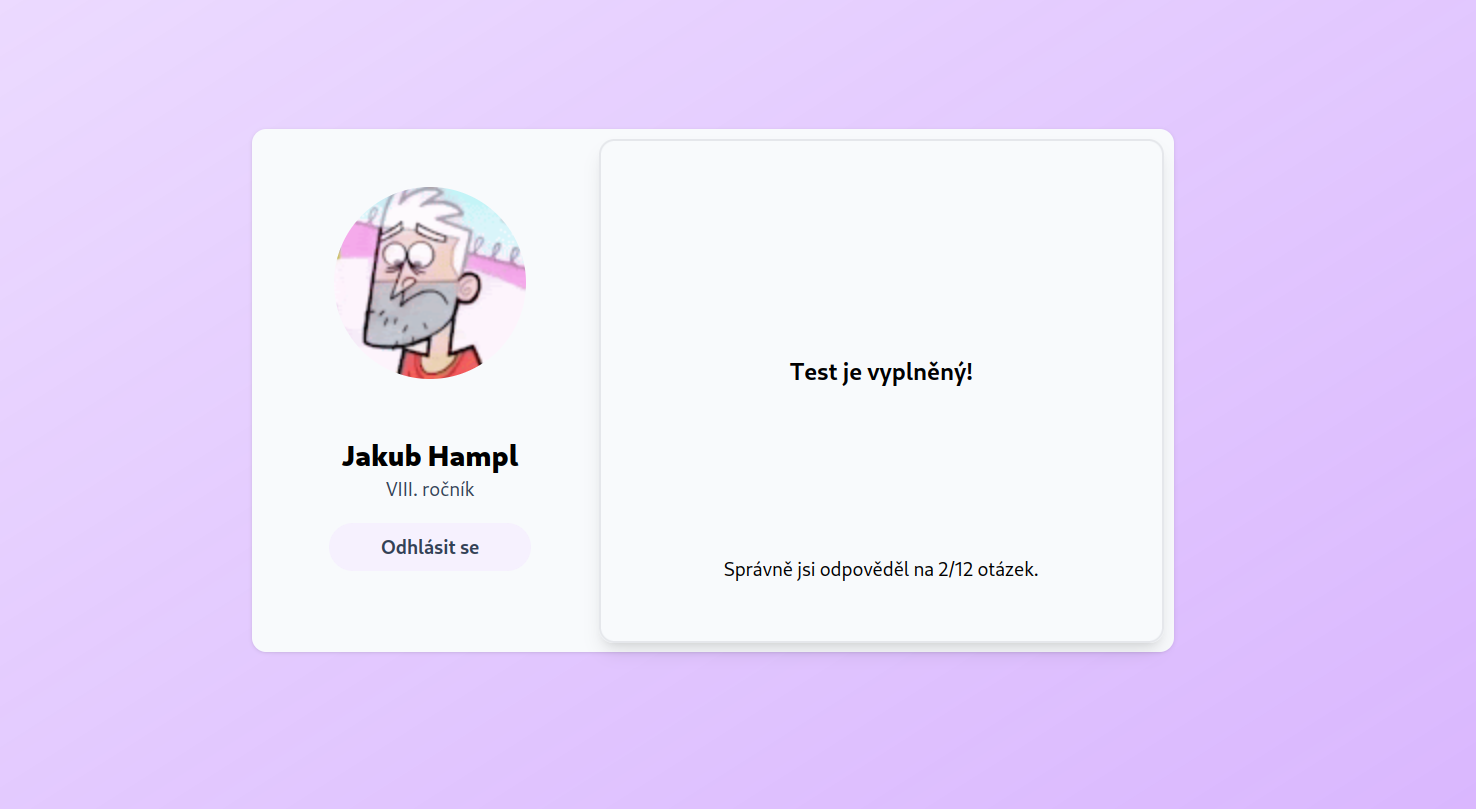
\includegraphics[width=350px]{images/01design/filled-out.png}
    \caption{Hlavní stránka s výsledky po odevzdání testu.}
\end{figure}

V případě, že žák na testování chyběl a stránku si zobrazí poté, co je test učitelem ukončen, zobrazí se mu tato informační stránka.

\begin{figure}[H]
    \centering
    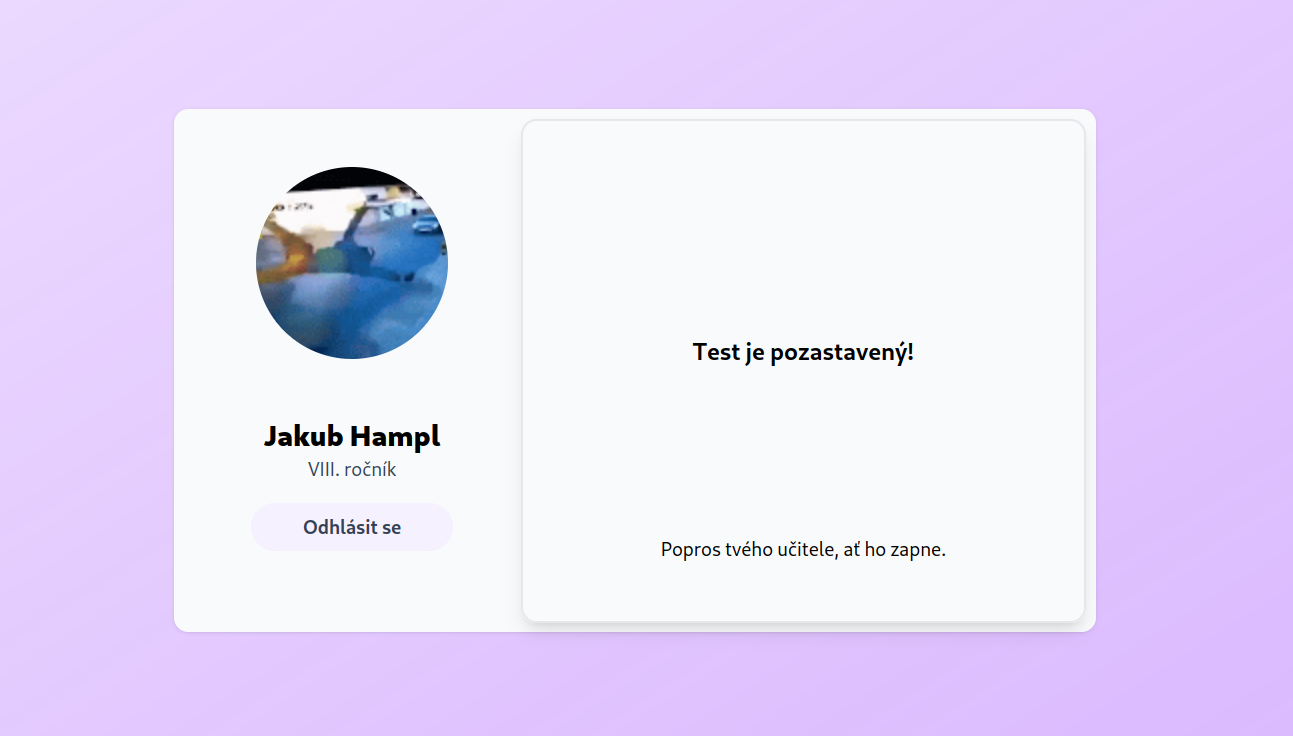
\includegraphics[width=350px]{images/01design/pending.png}
    \caption{Hlavní stránka s informací o pozastavení testu.}
\end{figure}

\section{Žákovské rozhraní}

Žákovské rozhraní slouží k vyplňování vygenerovaných testů. Pro každý ročník je předem nastavený čas a počet otázek různých obtížností (vizte ODKAZ). Z banky otázek je podle těchto kritérií několik náhodně vybráno a zobrazeno. Otázky mohou být různého druhu, ale u každé otázky je vždy na výběr ze čtyř možností z nichž právě jedna je správná. V pravém horním rohu každé otázky lze slabě vidět ID otázky (pro usnadnění komunikace s učitelem, například pokud student v otázce najde chybu).

\begin{figure}[H]
    \centering
    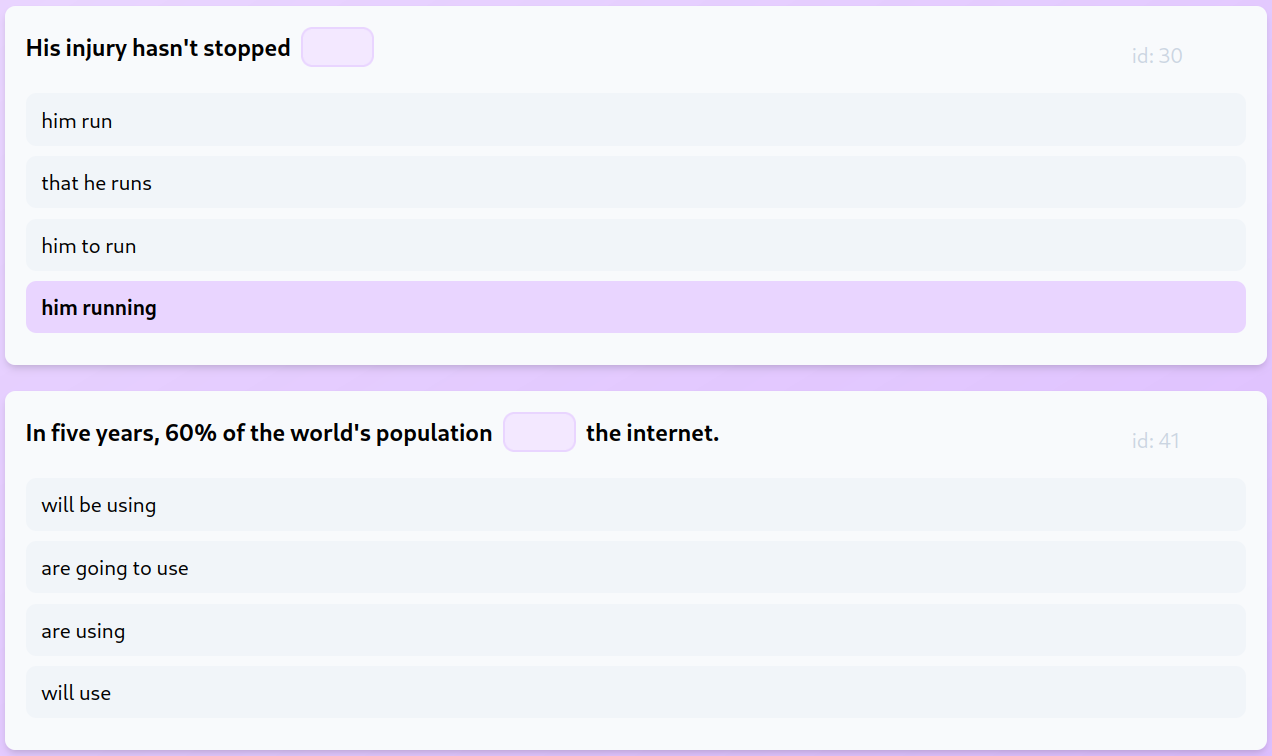
\includegraphics[width=400px]{images/01design/otazky.png}
    \caption{Dvě vygenerované otázky. Tmavě fialové ohraničení značí výběr.}
\end{figure}

\begin{figure}[H]
    \centering
    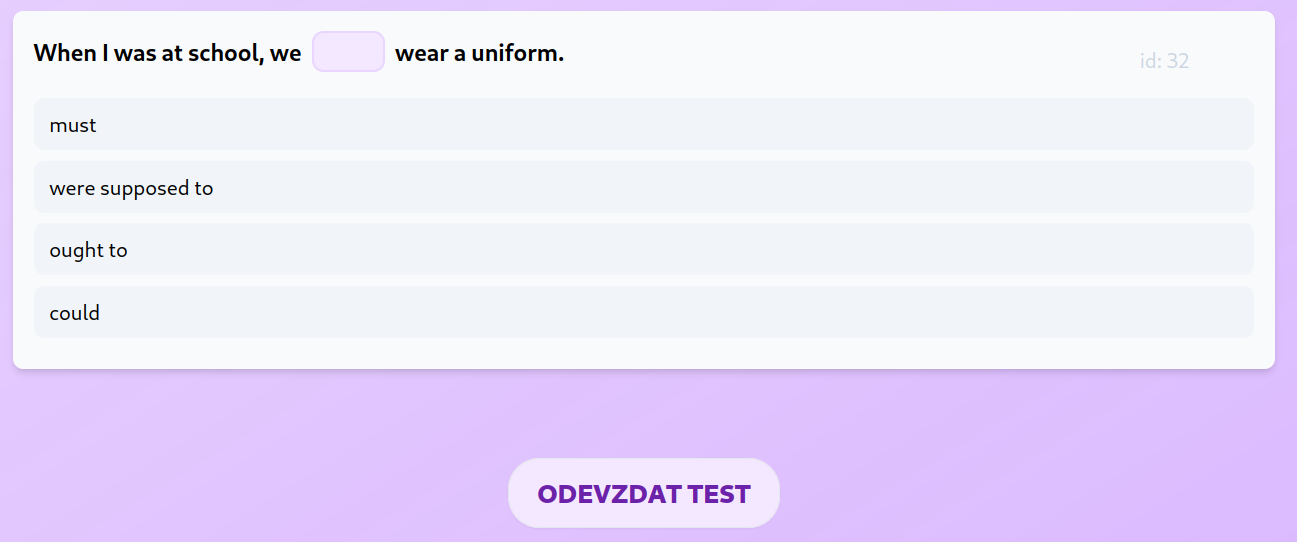
\includegraphics[width=400px]{images/01design/submit.png}
    \caption{Otázka a tlačítko pro odevzdání testu.}
\end{figure}

Po vyplnění testu může žák test odevzdat stisknutím tlačítka. Pokud tak neučiní do konce časového limitu, test se odevzdá sám. Po odevzdání testu je uživatel přesměrován zpět na hlavní stránku.

\section{Učitelské rozhraní}
\label{sec:admin}

Učitelské rozhraní je poměrně komplikované, proto je rozdělené do několika částí. V těchto částech se lze navigovat pomocí takzvaného \enquote{navbaru}, který se nachází v horní části obrazovky.

\begin{figure}[H]
    \centering
    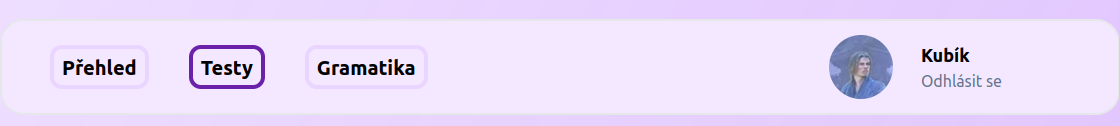
\includegraphics[width=400px]{images/01design/navbar.png}
    \caption{Navbar v učitelském rozhraní.}
\end{figure}

V jeho levé části můžeme přepínat do různých částí programu; aktuálně vybranou část značí fialový obrys. V pravé části lze vidět uživatelské jméno a možnost odhlásit se.

Po přihlášení se uživatel dostane do záložky \enquote{Přehled}, kde je prozatím vidět pouze aktuální počet spuštěných testů.

\subsection{Testy}

Tato sekce programu slouží ke správě testů a k stahování zpracovaných výsledků.

\begin{figure}[H]
    \centering
    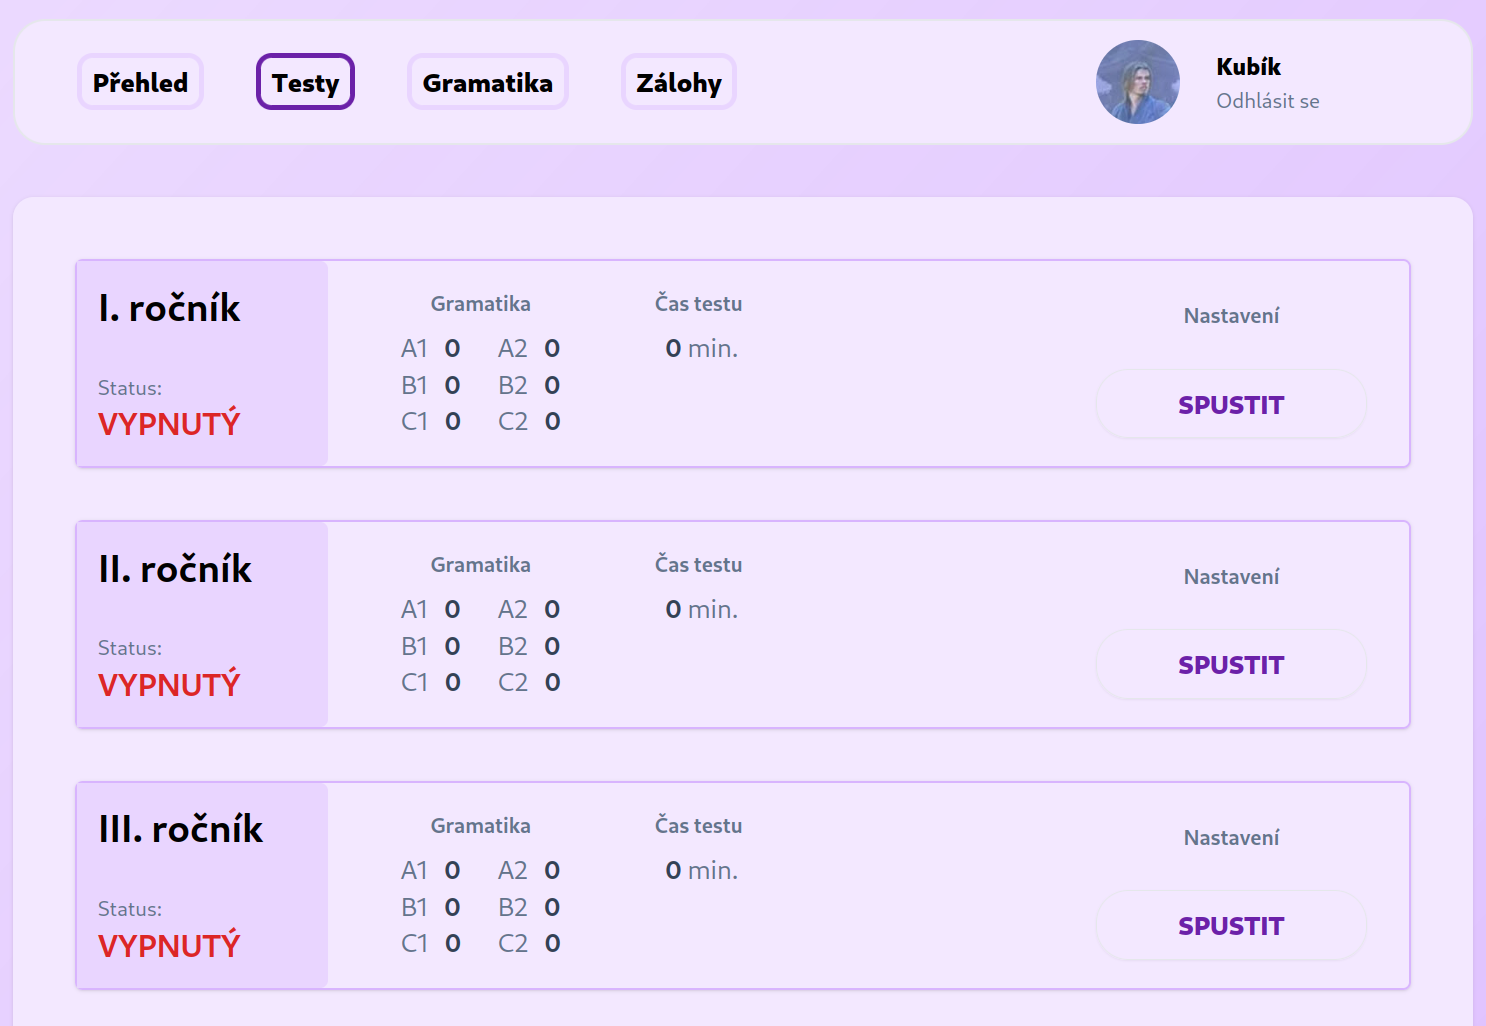
\includegraphics[width=400px]{images/01design/tests.png}
    \caption{Sekce Testy.}
\end{figure}

Při prvotním spuštění programu se automaticky vygeneruje osm testů (pro osm ročníků) s identickým výchozím nastavením. 

\begin{figure}[H]
    \centering
    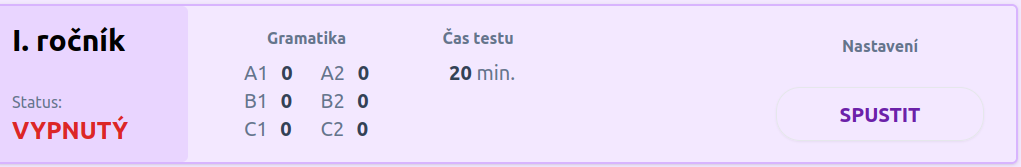
\includegraphics[width=400px]{images/01design/test.png}
    \caption{Detail komponentu testu.}
\end{figure}

V levé části se nachází číslo ročníku a status testu (\M{VYPNUTÝ}, \M{AKTIVNÍ} a \M{VYPLNĚNÝ}). V sloupci gramatika lze vidět počet použitých otázek pro každou jazykovou obtížnost. V sloupci čas testu lze vidět časový limit v minutách. Úplně vpravo pak tlačítka pro nastavení a spuštění testu.

\begin{figure}[H]
    \centering
    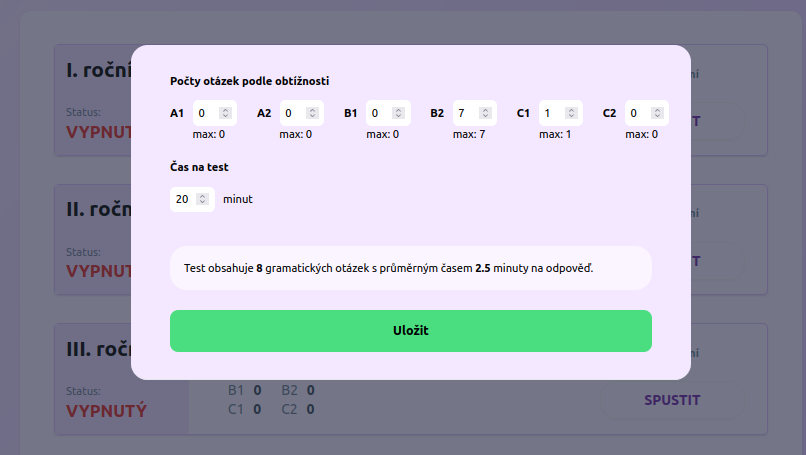
\includegraphics[width=400px]{images/01design/test-modal.png}
    \caption{Modální okno nastavení testu.}
\end{figure}

V modálním\footnote{Modální okno je typ uživatelského rozhraní, které vynucuje interakci s uživatelem, dokud není dokončena nebo zrušena. Tato okna se často zobrazují před ostatním obsahem na obrazovce.} okně nastavení lze změnit hodnoty pro použití otázek pro každou jazykovou obtížnost, níže i čas na test. Všechny zadané informace jsou shrnuty ve větě, která se během zadávání dat živě aktualizuje.

Tlačítko \M{Uložit} je zde spíše pro efekt, protože se stejně vše po zavření okna automaticky uloží.

Po zmáčknutí tlačítka \M{Spustit} se test spustí, což je reflektováno v statusu testu a v zablokování možnosti nastavení. V tomto stavu máme pouze možnost test zastavit.

\begin{figure}[H]
    \centering
    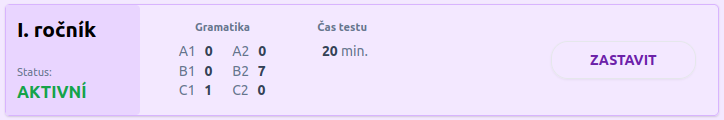
\includegraphics[width=400px]{images/01design/test-running.png}
    \caption{Detail spuštěného testu.}
\end{figure}

Po zastavení testu je status \M{VYPLNĚNÝ}. Z tohoto stavu lze test znovu spustit tlačítkem \M{Restartovat} (toto je například potřeba, pokud během rozřazovacích testů někdo chyběl, což je poměrně pravděpodobné), \M{Smazat výsl}{edky} (tato možnost test dostane zpět do stavu \M{VYPNUTÝ} a je nevratná) a nebo si stáhnout výsledky ve formátu \M{.xlsx} (Excel tabulka).

\begin{figure}[H]
    \centering
    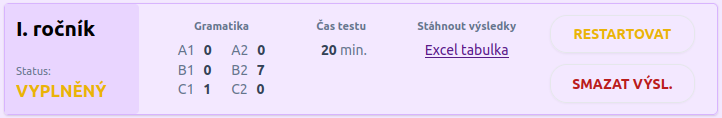
\includegraphics[width=400px]{images/01design/test-filled.png}
    \caption{Detail vyplněného testu.}
\end{figure}

Výsledná tabulka má sloupce pro jméno, e-mail, procentuální úspěšnost, získané body a ID špatně zodpovězených otázek (vizte ODKAZ). Řádky jsou seřazeny sestupně podle úspěšnosti.

\subsection{Gramatika}

Sekce Gramatika slouží k upravování gramatických otázek. Sestává se ze seznamu uložených otázek v databázi. V rychlém náhledu můžeme vidět text otázky, správnou odpověď, jazykovou úroveň otázky a ID. V horním pravém rohu této sekce se nachází tlačítko pro vytvoření nové otázky. Stejné tlačítko se nachází i na konci seznamu.

\begin{figure}[H]
    \centering
    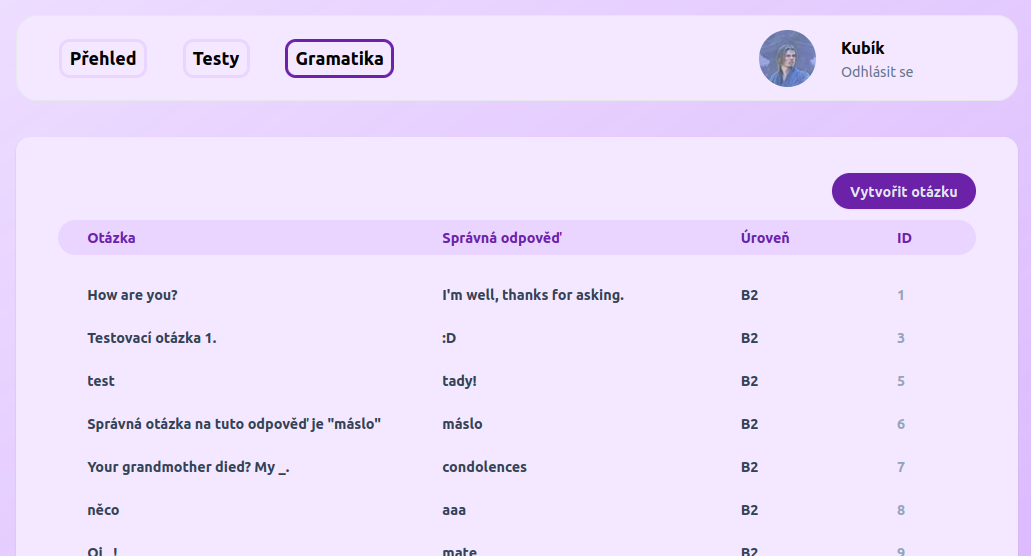
\includegraphics[width=400px]{images/01design/grammar.png}
    \caption{Sekce Gramatika.}
\end{figure}

Po kliknutí na otázku se otevře modální okno s nastavením dané otázky. Při kliknutí na tlačítko pro vytvoření otázky se otevře stejné okno, akorát nevyplněné. Zde je potřeba vyplnit text otázky, správnou odpověď, tři špatné odpovědi a vybrat jednu z jazykových obtížností. 

\begin{figure}[H]
    \centering
    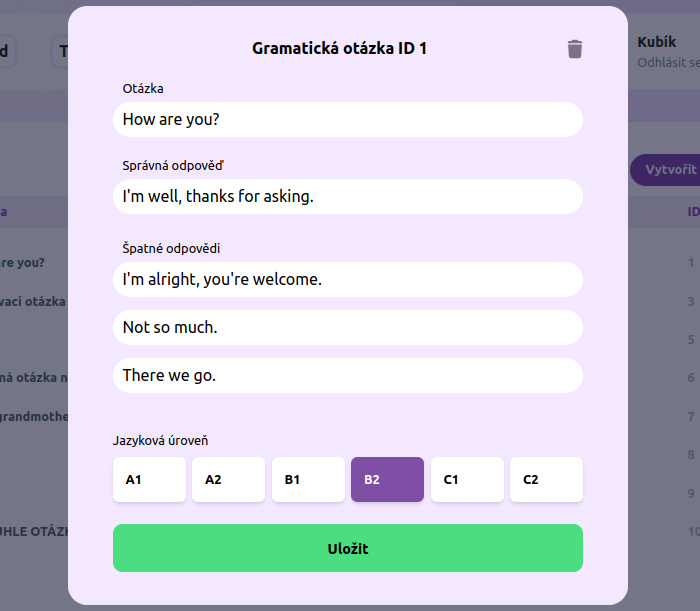
\includegraphics[width=400px]{images/01design/question.png}
    \caption{Modální okno nastavení gramatické otázky.}
\end{figure}

Program automaticky kontroluje správnost zadaných údajů -- zdali se nějaká ze špatných odpovědí neshoduje se správnou a zdali jsou všechna políčka vyplněná. Výchozí hodnota jazykové obtížnosti je A1.

\begin{figure}[H]
    \centering
    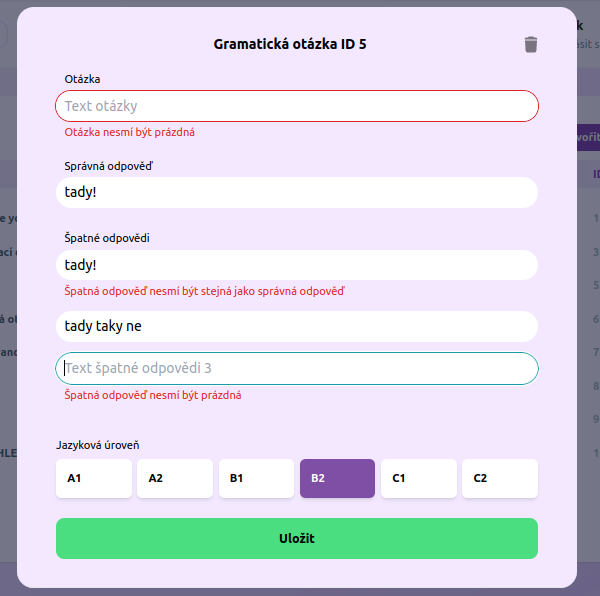
\includegraphics[width=400px]{images/01design/question-bad.png}
    \caption{Modální okno nastavení gramatické otázky s nesprávně vyplněnými hodnotami.}
\end{figure}

Pokud nejsou všechny pole vyplněna správně, nelze otázku uložit. Stále je však možné otázku smazat kliknutím na ikonku odpadkového koše v pravém horním rohu modálního okna.

\section{O Programu}

Na hlavní stránce se na spodní straně obrazovky nachází odkaz na informace \M{O programu}. Nachází se zde stručný popis toho, o čem program je, kde lze nalézt zdroj programu a kdo je aktuální správce programu (nastavitelné v konfiguraci, vizte \ref{sec:config})

\begin{figure}[H]
    \centering
    
\includegraphics[width=400px]{images/01design/about.png}
    \caption{Stránka O programu.}
\end{figure}
	\hypertarget{Technologie}{\chapter{Technologie}}

\section{Požadavky}

Důležitým uvážením při tvorbě projektu bylo výběr licence. Nakonec jsem se rozhodl pro použití licence GNU GPLv3, která je standardem takzvaných copyleft\footnote{Copyleft licence je typem licence pro software a jiný obsah, který umožňuje uživatelům volně používat, upravovat a sdílet software, přičemž vyžaduje, aby všechny odvozené verze byly také licencovány pod stejnými podmínkami. Tím zajišťuje, že software zůstane svobodným.} licencí.

Volba licence je důležitá, protože přímo ovlivňuje, jak se se softwarem může zacházet. GPLv3 mimo jiné zaručuje, že tento projekt navždy zůstane open-source; kdokoliv může prozkoumat, upravit a dále (pod stejnou licencí) sdílet zdrojový kód.\cite{choosealicense}

Dalšími podmínkami byla jednoduchost používání a aktuálnost různých nástrojů, programů a knihoven -- cílem bylo použít moderní (avšak osvědčené), aby program stárnul co možná nejpomaleji.

\subsection{Stack}

Dnes existuje nepřeberně způsobů, jak vytvořit full-stack\footnote{Full-stack označuje kompletní řešení, často za použití serverové i klientské aplikace.} aplikaci a vybrat mezi nimi není jednoduché. Mimoto je tyto technologie potřeba často kombinovat; této kombinaci se nazývá stack. Stack určuje, jak aplikaci vyvíjíme a jaké prostředky nám jsou dostupné. Stack si lze vytvořit sám dle vlastního uvážení a potřeb, nebo využít nějaký volně dostupný, který už je ozkoušený a důvěryhodný.

Mojí volbou se stal \M{T3 Stack}, který kombinuje několik populárních technologií, které jsou blíže popsány níže. Zároveň je však poměrně tvárný a lze ho jednoduše přizpůsobit potřebám projektu.\cite{t3stack}

Jedno z prvních rozhodnutí, které musí člověk při tvorbě projektu udělat je samotný výběr programovacího jazyka. Posledních pár let se většina vývoje soustředí kolem jazyka \M{TypeScript}, který je typovanou\footnote{Typy v programovacím jazyce definují struktury, ve kterých se mimo jiné dají ukládat data. Pokud předem víme, jak tyto struktury vypadají, dá se jednodušeji při programování vyhnout chybám.} variantou jazyka \M{JavaScript}. \M{T3 Stack} ho automaticky používá. 

Framework je jakási nadstavba nad programovacím jazykem a má proces vytváření webových aplikací usnadnit. Při tvorbě webové aplikace fungují jako páteř, na které stojí vše ostatní. \M{T3 Stack} přichází s frameworkem \M{Next.js}, který je sám o sobě nadstavbou nad populárním frameworkem \M{React}. Nabízí mnoho funkcí, jmenovitě například možnost výběru stylu renderování stránky, automatické optimalizace a různé další funkcionality.\cite{nextjs}

% TODO: TRPC??

Databáze je další klíčovou součástí jakékoli větší aplikace. Pro tento projekt jsem zvolil \M{PostgreSQL}; jedná se o jeden z nejvšestranějších volně dostupných databázových systémů.

\M{T3 Stack} přichází s knihovnou \M{Prisma}, která komunikaci s databázi usnadňuje například tím, že pro TypeScript generuje typy podle definovaného schéma.

Na rozdíl od jiných populárních CSS frameworků, jako je například \M{Bootstrap} nebo \M{Skeleton} se \M{TailwindCSS} liší tím, že nenabízí již předem připravené komponenty, ale pouze profesionály definované CSS třídy. Vývojář díky tomu není žádným způsobem omezován.\footnote{Navíc, pokud je člověk ve tvorbě webů zběhlý, na první pohled dokáže poznat připravené komponenty z populárních CSS  frameworků, což je vzhled, kterému jsem se chtěl vyvarovat.}\cite{tailwind} \M{TailwindCSS} je automaticky obsažen v \M{T3 Stack}u.

Autentifikace je při tvorbě webových aplikací častým úskalím, proto \M{T3 Stack} automaticky přichází s \M{NextAuth.js}, což je rozšíření pro použitý framework \M{Next.js}. Umožňuje přihlašování s Google účtem, což je pro tuto aplikaci potřeba. Jedná se o léta používaný standard, což je u což je u bezpečnostně kritického komponentu jedna z žádaných vlastností. Zároveň jsou všechny kritické bezpečnostní chyby hlášeny na amerických státních stránkách NIST.

Sestavený kód je spouštěn pomocí \M{Node.js} za pomocí balíčkovacího programu \M{NPM}. Zároveň je možné celý program spolu s databázovým systémem spustit v \M{Docker} kontejnerech.

Program je verzován pomocí verzovacího systému \M{Git}.

Všechny výše zmíněné technologie jsou dostupné pod open-source licencemi.

\section{Program}

Program je poměrně rozsáhlý, proto je pro přehlednost rozdělen do několika souborů a složek. Všechny konfigurační soubory se nacházejí v kořenové cestě aplikace. Všechny soubory týkající se databáze, včetně migrací\footnote{Migrace je sql soubor který definuje postupné změny databáze během vývoje.} a schématu, jsou ve složce \M{/prisma/}. Všechny statické soubory, jako jsou například obrázky a ikony jsou ve složce \M{/public/} (toto je složka, kterou \M{Next.js} automaticky detekuje a všechny soubory uvnitř ní zveřejní v sestavené verzi aplikace). Složka \M{/src/} obsahuje samotný zdrojový kód.

\subsection{Konfigurace}
\label{sec:config}

Protože je v programu použito hodně nástrojů, je potřeba mnoha konfiguračních souborů.

\M{package.json} definuje použité knihovny a různé scripty\footnote{Script je typicky malý kus kódu, který nijak nezasahuje do funkčnosti aplikace, ale vypomáhá při jejím vývoji.}; tento soubor využívá balíčkovací systém \M{NPM} při instalaci potřebných balíčků. \M{tailwind.config.cjs}, \M{prettier.config.cjs} a \M{postcss.config.cjs} nastavují funkčnost \M{Tailwind}u. \M{next.config.mjs} a \M{next-env.d.ts} konfigurují funkčnost \M{Next.js}. Soubor \M{.gitignore} definuje, jaké soubory má \M{Git} ignorovat.

Konfigurace samotného programu je uložena v souboru \M{.env}. Tento soubor není v repozitáři přítomen, protože obsahuje citlivé informace (přístupové údaje k databázi aj.); místo toho je přítomen soubor \M{.env-example}, kde jsou všechny nastavitelné hodnoty popsány a nevyplněny. Níže následuje úryvek z tohoto souboru.

\indent

\hrule
\begin{verbatim}
# VARIABLE INFO
NEXT_PUBLIC_SUBTITLE="Rozřazovací testy pro [jméno školy]"
NEXT_PUBLIC_REPOSITORY="https://github.com/chamik/rozrazovak"
NEXT_PUBLIC_CONTACT_EMAIL="aktualni-administrator@example.org"

# Teacher email adresses (comma separated)
TEACHER_EMAILS=ucitel@gjp-me.cz,obcan-k@email.cz

# Prisma
POSTGRES_USER=postgres
POSTGRES_PASS=supertajneheslo
POSTGRES_DB=rozrazovak

# Next Auth Google Provider
GOOGLE_CLIENT_ID=
GOOGLE_CLIENT_SECRET=
\end{verbatim}
\hrule

Kvůli bezpečnosti nejsou ve výchozím stavu tyto proměnné přístupné v klientské aplikaci. Proto je potřeba k názvu těch, které na klientu chceme používat, na začátek přidat \enquote{\M{NEXT\_PUBLIC\_}}. \M{Next.js} poté tyto proměnné v klientské aplikaci zpřístupní.

Pro usnadnění spouštění programu lze projekt spustit v Docker kontejneru. Soubor \M{Dockerfile} definuje, jak program sestavit a spustit. Soubor \M{docker-compose.yml} poté definuje, jak se má spustit databáze spolu s programem a jak mezi sebou komunikují. \cite{docker}

Script \M{start.sh} podle nastavení při každém spuštění provede migrace databáze a končeně spouští program.

\subsection{Databáze}

Schéma databáze je definované pomocí souboru \M{prisma/schema.prisma}. Obsahuje definice uživatelů, testů, odpovědí, aktuálních přihlášení aj. (vizte obrázek \ref{schema}) Jedná se o soubor se speciálním zápisem, který následně \M{Prisma} používá k vytváření SQL migrací, Typescript typů atd. Díky této funkcionalitě v programu není ani jeden ručně psaný řádek SQL kódu.

Výhodou tohoto přístupu je, že \M{Prisma} dokáže převádět tento obecný zápis a dotazy na specifické verze SQL podle použité databáze. \cite{prisma} Níže následuje úryvek schématu.

\begin{lstlisting}[language=Prisma, caption={Úryvek schéma databáze}]
model Question {
    id            Int          @id @default(autoincrement())
    languageLevel Int          @default(0)
    questionText  String       @default("")
    rightAnswer   String       @default("")
    wrongAnswers  String[]     @default(["", "", ""])
    questionType  QuestionType @default(GRAMMAR)
    pointAmount   Int          @default(1)

    answers Answer[]
}

enum QuestionType {
    GRAMMAR
    READING
    LISTENING
}
\end{lstlisting}

\begin{figure}[H]
    \centering
    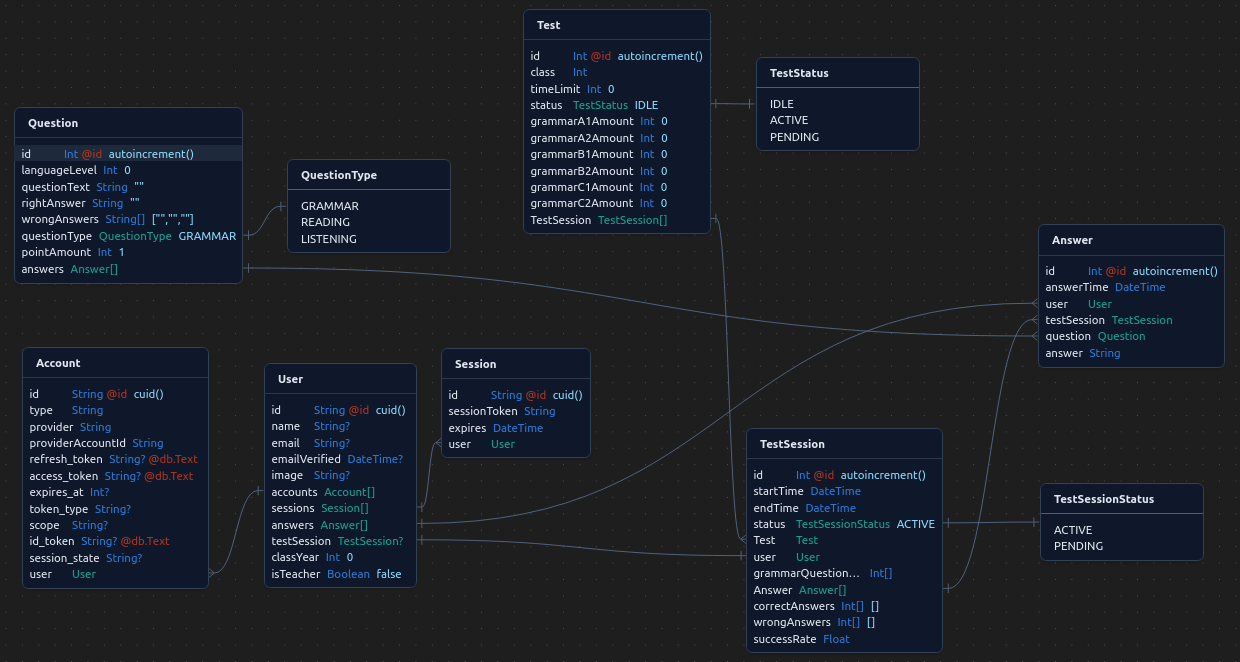
\includegraphics[width=420px]{images/02technologie/schema.png}
    \caption{Vizualizované schéma databáze. Každý modrý blok popisuje jednu tabulku. V tabulce se nachází jména sloupců společně s jejich typy. Šedé čáry značí relace.}
    \label{schema}
\end{figure}

Během vývoje se schéma databáze měnilo. Při každé změně byla vytvořena migrace, která změnu přesně popisuje. Díky tomu lze program vracet do různých fází vývoje a aktualizovat živou\footnote{Takzvaná živá databáze je databáze s produkčními daty. Při vývoji se používá databáze lokální, aby případně nedošlo ke katastrofické ztrátě dat.} databázi bez větších problémů. Všechny migrace se nachází ve složce \M{prisma/migrations/}.

\subsection{Přihlašování}
\label{sec:login}

Boilerplate\footnote{Boilerplate je opakující se nebo standardní kód, který je často používán v různých částech softwaru a aplikací. Jedná se o kód, který obsahuje základní strukturu a funkce.} kód pro přihlašování přichází s \M{T3 Stack}em už připravený, je však upraven tak, aby vyhovoval požadavkům projektu -- specificky aby aplikace umožňovala přihlašování se školním Google účtem.

Specifická implementace se nachází v \M{src/pages/api/auth/[...nextauth].ts}. Při přihlášení si program kontroluje použitou e-mail adresu -- nejdříve pokud se nachází v seznamu učitelů (vizte \ref{sec:config}), v takovém případě uživateli přidělí roli učitele s přístupem do učitelského rozhraní (vizte \ref{sec:admin}). 

Pokud ne, program se ujistí, že je e-mail součástí školní domény. Poté je díky specifické konvenci GJP-ME dávat žákům e-mailové adresy ve formátu \M{[rok nástupu na školu][typ studia][pořadí žáka v abecedním seznamu]@gjp-me.cz} schopen získat rok nástupu žáka a podle toho vypočítat, v jakém ročníku se aktuálně nachází (vizte níže). Všechny tyto údaje jsou uloženy do databáze.

\begin{lstlisting}[language=JavaScript,caption={Zjištění aktuálního ročníku uživatele}]
function parseUserLevel(email: string) {
    const emailId = email.split('@')[0];
    
    const date = new Date();
    const currentYear = date.getFullYear();
    const currentMonth = date.getMonth();
    
    const userYear = 2000 + parseInt(emailId!.slice(0, 2)!);
    
    let level = 0
    if (emailId?.slice(2, 4) == '08')
        level = currentYear - userYear;
    else
        level = currentYear - userYear + 4;
    
    if (8 <= currentMonth && currentMonth <= 11 )
        level += 1;
    
    return level;
}
\end{lstlisting}

Aby bylo přihlašování přes Google účet možné, je potřeba svoji aplikaci registrovat v Google Developer Console. Zde je možné editovat, k jakým údajům uživatele má aplikace přístup (v tomto případě pouze ke jménu a e-mailu), název aplikace zobrazený uživateli aj. Také je zde potřeba správně nastavit callback adresu -- kam Google uživatele přesměruje po přihlášení -- a potvrzené zdroje JavaScriptu.

\begin{figure}[H]
    \centering
    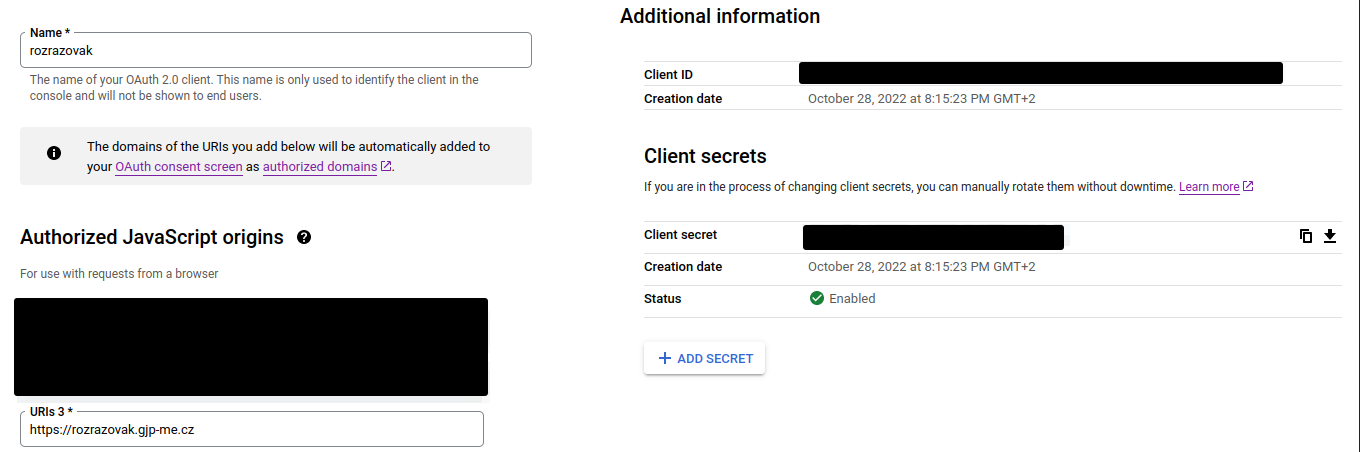
\includegraphics[width=420px]{images/02technologie/google-console.png}
    \caption{Redigovaný snímek obrazovky z Google Developer Conosle.}
\end{figure}

Po správném nastavení a potvrzení administrátorem organizace podle použité domény aplikace je na této stránce možné získat \M{CLIENT\_ID} a \M{CLIENT\_SECRET}, které je potřeba vyplnit v konfiguračním souboru aplikace (vizte \ref{sec:config}).

K potvrzení identity uživatele se používá protokol OAuth 2.0, který \M{NextAuth.js} automaticky zpracuje a vývojáři zpřístupní relevantní údaje, jako je například právě e-mail a jméno.

\begin{figure}[H]
    \centering
    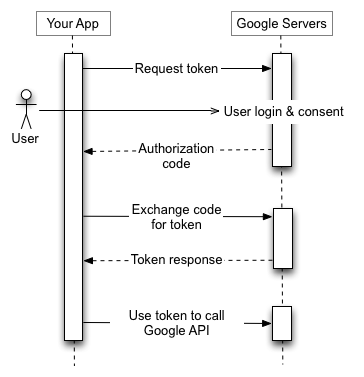
\includegraphics[width=200px]{images/02technologie/google-auth.png}
    \caption{Schéma komunikace aplikace se servery Googlu během přihlašování. Sdíleno Googlem. \cite{google-auth}}
\end{figure}

Pokud celý tento proces proběhl úspěšně, je uživatel přesměrován zpět na hlavní stránku (vizte \ref{sec:login-design}). Pokud ne, uživateli je sděleno, že přihlašování neproběhlo úspěšně a je přesměrován na interní stránku \M{NextAuth.js}, kde má možnost se zkusit přihlásit znovu.

\section{API}
\label{api}

Přestože se celý program zapisuje do jedné souborové struktury, běží některý kód pouze na serveru. Tento kód se nachází v \M{/src/server/}. \M{Next.js} při kompilaci spojí všechny typescript zdrojové soubory a vytvoří z nich jeden javascript program. Tento program spustí svůj webserver na portu definovaném v konfiguraci (vizte ODKAZ). API\footnote{API (application programming interface; česky rozhraní pro programování aplikací) definuje možnosti vzájemné komunikace aplikací (v tomto případě serveru a klienta).} samotné je dostupné na cestě \M{[doména]/api/trpc/} -- tato adresa je definována v \M{/src/utils/tprc.ts} a je na ni možné posílat tradiční json požadavky. Toto API využívá v pozadí i aplikace.

API je rozdělené do dvou hlavních částí s různými pravomocemi -- uživatelské a učitelské. Uživatelské je dostupné všem přihlášeným uživatelům. Učitelské je dostupné pouze oprávněným uživatelům -- server si zkontroluje, pokud je u uživatele v databázi vyplněná kolonka \M{isTeacher}. Tento kód se nachází v \M{/src/server/trpc/trpc.ts} a jeho ukázka je níže.

\begin{lstlisting}[language=JavaScript,caption={Kontrola přístupu do učitelského rozhraní}]
const isTeacher = t.middleware(async ({ ctx, next }) => {
    if (!ctx.session || !ctx.session.user) {
        throw new TRPCError({ code: "UNAUTHORIZED" });
    }
    
    const user = await ctx.prisma.user.findFirst({ where: 
        { email: ctx.session.user.email }});

    if (!user || !user.isTeacher)
        throw new TRPCError({ code: "UNAUTHORIZED" });
    
    return next({
        ctx: {
        // infers the `session` as non-nullable
        session: { ...ctx.session, user: ctx.session.user },
        },
    });
});

export const teacherProcedure = t.procedure.use(isTeacher);
\end{lstlisting}

\subsection{Uživatelské API}
\label{userapi}

Uživatelské API se nachází v \M{/src/server/trpc/router/user.ts}. Definuje následující endpointy\footnote{API endpoint je specifický koncový bod nebo URL v rámci API, které představuje konkrétní operaci nebo zdroj poskytovaný daným rozhraním. V tomto případě každý endpoint reprezentuje jednu funkci na severu.}:

% TODO: tečky na konci řádků?
\begin{compactitem}
    \item getUserData -- vrátí informace o přihlášeném uživateli, aktuálním spuštěném testu a případně o vyplněném testu
    \item beginTest -- vygeneruje test pro daného uživatele, uloží do databáze ID použitých otázek a čas ukončení testu 
    \item getTestData -- navrátí náhodně zamíchaná vygenerovaná data testu, označí test za aktivní
    \item submitAnswer -- přijímá odpověď na otázku, kterou uloží do databáze
    \item submitTest -- potvrdí odevzdání testu, zablokuje další odevzdávání otázek. Zároveň test vyhodnotí a výsledky uloží do databáze
\end{compactitem}

Následuje ukázka endpointu \M{getTestData}

\begin{lstlisting}[language=JavaScript,caption={Endpoint getTestData}]
getTestData: protectedProcedure.query(async ({ ctx }) => {
    const user = await prisma.user.findFirst({ 
        where: { email: ctx.session.user.email },
    });

    if (!user)
        return;

    const sesh = await prisma.testSession.findFirst({
        where: { userId: user.id },
    })

    if (!sesh)
        return;

    const questionsIds = sesh.grammarQuestionsIds;
    const questions = await prisma.question.findMany({
        where: {
            id: { in: questionsIds }
        },
        select: {
            id: true,
            questionText: true,
            rightAnswer: true,
            wrongAnswers: true,
        },
    });

    const shuffled = shuffle(questions.map(x => ({
        id: x.id,
        questionText: x.questionText,
        answers: shuffle([x.rightAnswer, ...x.wrongAnswers]),
    })));

    const answers = await prisma.answer.findMany({
        where: {
        testSessionId: sesh.id,
        },
        select: {
        questionId: true,
        answer: true,
        },
    });

    return ({
        questions: shuffled,
        testSession: sesh,
        submittedAnswers: answers,
    });
}),
\end{lstlisting}

\newpage
\subsection{Učitelské API}
\label{adminapi}

Učitelské API se nachází v \M{/src/server/trpc/router/admin.ts}. Definuje následující endpointy:

\begin{compactitem}
    \item getAllQuestions -- navrátí obecné informace o všech otázkách v databázi
    \item getQuestionById -- získá detail otázky z databáze podle daného ID
    \item getTestById -- získá detail testu z databáze podle daného ID
    \item saveQuestion -- uloží nové údaje po editaci otázky do databáze (vizte ODKAZ)
    \item newQuestion -- vytvoří novou otázku s výchozími údaji a uloží ji do databáze
    \item getQuestionLevels -- vrátí počet otázek v databázi pro každou jazykovou obtížnost
    \item deleteQuestion -- odstraní otázku z databáze
    \item getAllTests -- navrátí obecné informace o všech testech v databázi.
    \item saveTest -- uloží nové údaje po editaci testu do databáze (vizte ODKAZ).
    \item deleteTest -- odstraní test z databáze (tento endpoint nelze spustit manuálně přes uživatelské rozhraní, používá se pouze interně)
    \item toggleTest -- označí test jako \M{AKTIVNÍ}, nebo \M{VYPLNĚNÝ}, podle jeho aktuálního stavu
    \item restartTest -- ze stavu \M{VYPLNĚNÝ} nevratně smaže data o vyplnění a vrátí ho do stavu \M{VYPNUTÝ}
    \item areTestRunning -- vrátí pravdivostní hodnotu pokud je alespoň jeden test ve stavu \M{AKTIVNÍ}, nebo \M{VYPLNĚNÝ}
    \item downloadResults -- vygeneruje excel tabulku do které přidá data výsledků daného testu převedenou do formátu Base64
\end{compactitem}

Následuje kód pro endpoint \M{downloadResults}

\begin{lstlisting}[language=JavaScript,caption={Endpoint downloadResults}]
downloadResults: teacherProcedure.input(z.object({testId: z.number()})).mutation(async ({ input }) => {
    const test = await prisma.test.findFirst({ where: { id: input.testId }});
    if (!test) return;
    
    if (test.status != TestStatus.PENDING) return;

    const results = await prisma.testSession.findMany({
      where: {
        testId: input.testId,
      }, 
      orderBy: {
        successRate: "desc",
      }
    });

    if (!results) return;

    const users = await prisma.user.findMany({
      where: {
        id: {
          in: results.map(x => x.userId),
        }, 
      },
    })

    const workbook = new Workbook();
    const worksheet = workbook.addWorksheet('Vysledky testu')

    worksheet.columns = [
      { header: "Jmeno", key: "name", width: 25 },
      { header: "E-mail", key: "email", width: 30 },
      { header: "Body gr.", key: "points_gr", width: 10},
      { header: "Uspesnost gr.", key: "success_gr", width: 15 },
      { header: "ID spatnych odpovedi gr.", key: "wrong_ids_gr", width: 40 },
    ];

    const usrs = users.reduce((acc, user) => {
      acc[user.id] = user;
      return acc;
    }, {} as { [key: string]: typeof users[0] });

    results.forEach(s => {
      worksheet.addRow({
        name: usrs[s.userId]?.name ?? "Bezejmenny",
        email: usrs[s.userId]?.email ?? "???",
        points_gr: s.correctAnswers.length,
        success_gr: (s.successRate * 100).toFixed(1) + "%",
        wrong_ids_gr: s.wrongAnswers.join(" "),
      });
    });

    const bf = await workbook.xlsx.writeBuffer();
    const st = Buffer.from(bf).toString("base64");

    return st;
}),
\end{lstlisting}

\section{Komponenty a stránky}

Vysrat se na to?
	
	
	
	%%% Závěr
	\chapter*{Závěr}
\addcontentsline{toc}{chapter}{Závěr}

Opravdový provoz aplikaci čeká až na začátku příštího školního roku, ovšem podle testování a průběžného používání práce splnila svůj cíl -- vyvinula se v intuitivní, příjemně vypadající aplikaci, která automaticky a férově testuje žáky a vyhodnocuje jazykové rozřazovací testy.

Aplikace vyhovuje požadavkům angličtinářů a s jejich souhlasem se na našem gymnáziu bude aktivně využívat k testování žáků.

V budoucnu bych rád získal zpětnou vazbu od studentů, kteří budou aplikací otestováni a provedl úpravy na základě jejich podnětů.

Toto téma si mimo Středoškolské odborné činnosti vybírám i jako maturitní práci z programování, tudíž stále nabízí další výzvy, zejména přidání sekcí na testování čtení a poslechu. I přesto věřím, že je dostatečně vyvinutá na to, aby se dala běžně používat a nebyla pouhou přítěží. Při troše štěstí bude \textit{Rozřazovák} ještě dlouhá léta dobře sloužit, než také podlehne digitálnímu stáří.

Zdroj programu a návod k jeho spuštění lze nalézt na těchto odkazech:

\href{https://chamik.eu/rozrazovak}{chamik.eu/rozrazovak},\newline
\href{https://github.com/chamik/rozrazovak/}{github.com/chamik/rozrazovak}.

	\pagenumbering{gobble}
	\newpage
	\printbibliography[title=Literatura]
	\nocite{*}
	\addcontentsline{toc}{chapter}{Literatura}
	\renewcommand{\baselinestretch}{1.5} 

	%\lstlistoflistings
	%%%\addcontentsline{toc}{chapter}{Seznam programů}{\linespread{1}\selectfont}
	
	
	\listoffigures
	\addcontentsline{toc}{chapter}{Seznam obrázků}{\linespread{1}\selectfont}
	
	

	
\end{document}
